\section{Challenges and Problem Formulation}
\label{sec:problemformulation}

% Introduce the content of this section
In this section, we illustrate the challenges of band selection
in wireless network deployment and formulate the problem of band 
selection in mesh network deployments jointly using WiFi and white space bands. 
Further, we present a measurement-driven framework for estimating the 
mesh node number to serve the traffic demand of a given population.
 
\subsection{White Space Opportunity and Challenge}
\label{subsec:motivation}
% Propagation
Wireless propagation is the behavior of the signal loss characteristics 
when wireless signals are transmitted through the wireless medium.
The strength of the received signal depends on both the line-of-sight
path (or lack thereof) and multiple other paths that result from 
reflection, diffraction, and scattering from 
obstacles~\cite{andersen1995propagation}. The widely-used Friis
equation characterizes the received signal power $P_r$ in terms 
of transmit power $P_t$, transmitter gain $G_t$, receiver gain $G_r$, 
wavelength $\lambda$ of the carrier frequency, 
distance $R$ from transmitter to receiver, and path loss exponent 
$n$ according to~\cite{friis}:
\begin{equation}
\label{eq:friis}
P_r=P_t+G_t+G_r+10n \log_{10}\left( \frac{\lambda}{4\pi R}\right)
\end{equation}
Here, $n$ varies according to the aforementioned environmental 
factors with the value of two to five in typical outdoor 
settings~\cite{rappaport}.

% Existing Interference
%Wireless communication has changed the world since the day it was discovered.
%Wireless signals have filled up the world with different the frequency bands.
%These signals help people improve their lives as well as bringing interference
%to each other when they are in the same frequency band.
Despite sufficient levels of received signal, interference can cause channels
to be unusable (e.g., due to high levels of packet loss) or unavailable (e.g., 
due to primary users in cognitive radios~\cite{haykin2005cognitive}).
Prior work has worked to reduce interference levels via gateway deployment,
channel assignment, and routing~\cite{he2008optimizing,tang2005interference}.
The interference of a wireless network could be divided into two categories
according to the interferring source: {\it (i)} intra-network interference,
caused by nodes in the same network, and {\it (ii)} inter-network interference,
caused by nodes or devices outside of the network. Most of the existing works
try to reuce the intra-network interference without regard to the inter-network 
interference~\cite{si2010overview}. However, the existence of inter-network 
interference becomes an important problem when considering the availability
of white space bands.  While theoretical models describing inter-network 
interference exist, accurately characterizing a particular region must be done empirically.

% Explain multiband and activity level
When wireless devices operate in WiFi bands, the channel separation is relatively 
small (e.g., 22 MHz for the 2.4 GHz band). As a result, many works assume that
the propagation characteristics across channels are similar. However, with the
large frequency differences of WiFi and white space bands (e.g., multiple GHz),
propagation becomes a key factor in the deployment of wireless networks with both bands.
Here, a frequency band is defined as a group of channels which have
small separation meaning similar propagation characteristics.
In this work, we consider the diverse propagation and activity characteristics
for four total frequency bands: 450 MHz, 800 MHz, 2.4 GHz, and 5.2 GHz.
We refer to the two former frequency bands as white space bands and
the two latter frequency bands as WiFi bands.
The differences in propagation and spectrum utilization creates opportunity
for the joint use of white space and WiFi bands in wireless access networks according
to the environmental characteristics (e.g., urban or rural and downtown or residential)
of the deployment location.

% Network Constraint
Typically, the deployment of wireless access networks is subject to coverage and capacity
constraints for a given region. Coverage is defined with respect to the ability of
clients to connect to access points within their service area.  We use a coverage
constraint ratio of $95\%$ in this work for a target area~\cite{robinson2010deploying}.
Capacity is defined with respect to the ability of a network to serve the traffic 
demand of clients.  Spatial reuse allows improved capacity, but increases the cost
of deploying a network by increasing the total number of access points required.
Hence, for densely populated areas the greatest level of spatial reuse possible
is often desired.  In contrast, sparsely-populated rural areas have lower traffic
demand per unit area.  Thus, aggregating this demand with lower-frequency, white 
space bands could be highly effective in reducing the total number of access points 
required to achieve similar coverage and capacity constraints.  Moreover, since
less TV channels tend to be occupied in sparsely populated areas~\cite{msdatabase}, 
a larger number of white space bands can be leveraged in these areas.

% Make multiband challenges
%The broadcast nature of the wireless induces interferences, 
%as both Inter-network and Intra-network interferences. 
%Avoiding the Intra-network interference has been deeply explored in 
%many works~\cite{subramanian2008minimum,ramachandran2006interference,si2010overview}.
%However, few of them try to address the inter-network interference.
%Due to the distribution nature of the Inter-network interference,
%it is difficult to build a theoretic model describing and estimating the activities of existing
%wireless signals. Measurement is the best and probably the only way 
% to tell the Inter-network interference. 



% Spectrum utility vary across different areas
%Jointly using WiFi and white space band adapting different 
%demands of rural area and urban areas is a key issue in 
%multiband wireless network deployment. 
%Thus, in sparsely-populated rural areas, the lower frequencies of the white space 
%bands might be a better choice for wireless service in sparsely populated areas. 
%However, as the population and demand scales up (e.g., 
%for urban regions), the greater levels of residents traffic demands 
%might detract the white space bands from the 
%overall deployment strategy. In such urban areas, select channels in 
%spacial reusable WiFi bands might be more appropriate, 
%since the degree of inter-network interference is often  
%proportional to the population (due to the existence of greater TV channels).

%The activity of inter-network interference is hard to tell in formula. 
%But from our measurements and TV station database, its activity correlate to the population distribution~\cite{msdatabase}.
%Figure~\ref{fig:drivemap} depicts a map of the available white space channels with
%markers where we performed measurements in North Texas. To be representative of a broad range of 
%community types, we consider populations of approximately 25 times one another according to the
%2010 U.S. Census, Millsap (500), Weatherford (25k), and Dallas (1.25 M). 
%
%%FIXME - put in experiment section
%As an initial experiment, 
%we perform a drive test from Dallas to Weatherford with cruise control set to 60 MPH while on
%the highway.  
%Part of the result of in-field spectrum measurement is shown in Figure~\ref{fig:drivetest}.
%The measured RSSI of 450 MHz is strong in downtown Dallas, downtown Fort Worth;
%but has less signal activity in the urban and rural area between these cities.
%The low activity level detected in WiFi bands is due to the distance from highway is larger
%than the propagation range of an indoor wireless router whose transmitting power is limited.
%The map itself shows the available white space channels in DFW area, more green means
%more channels. Our in-field measurement matches the FCC restriction showing that less channels means
%more spectrum utility and tell the spectrum utility levels varying across population 
%distribution. We also collect measurements at more fixed locations as marked on the map to collect
%data for the spectrum utility calculation. 
%\begin{figure}
%%\vspace{-0.0in}
%\centering
%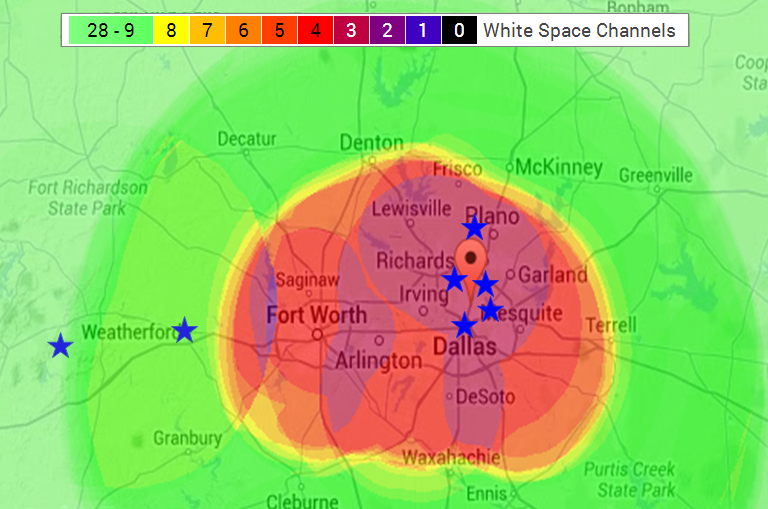
\includegraphics[width=74mm]{figures/drivemap}
%\vspace{-0.1in}
%\caption{DFW Metropolitan Measurement Location}                                                                 
%\label{fig:drivemap}
%\vspace{-0.1in}
%\end{figure}
%   
%\begin{figure}
%%\vspace{-0.0in}
%\centering
%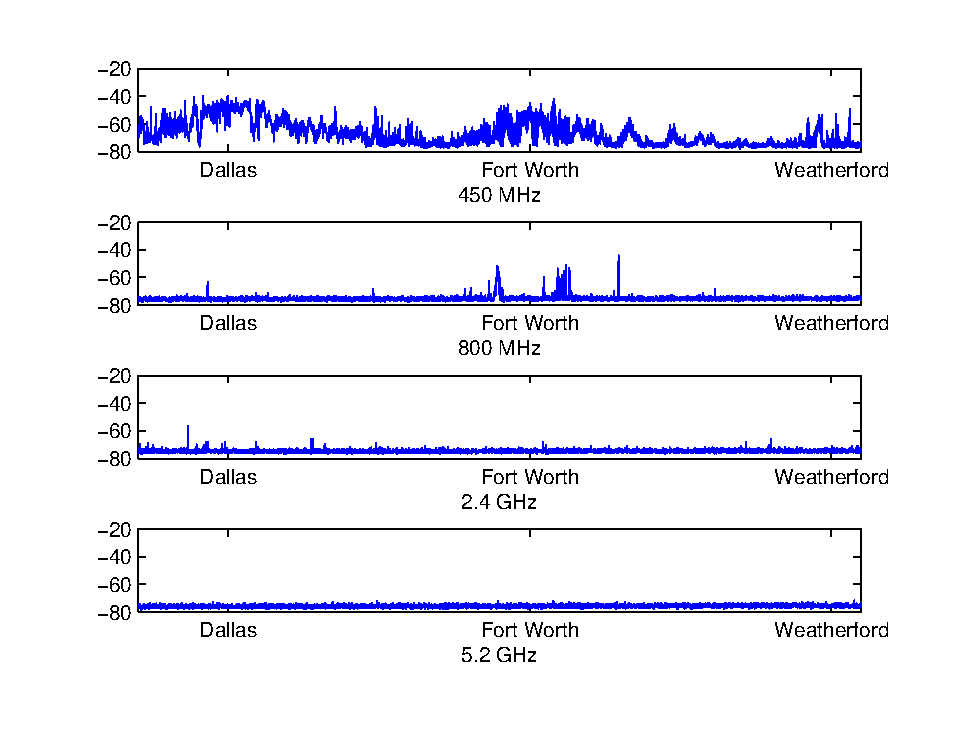
\includegraphics[width=94mm]{figures/drivetest}
%\vspace{-0.1in}
%\caption{Spectrum Activity In DFW}                                                                 
%\label{fig:drivetest}
%\vspace{-0.1in}
%\end{figure}
%
%% Fix location example claiming the activity is kind of stable
%Figure~\ref{fig:labact} depicts an example spectrum utility in activity level
%defined in~\ref{subsec:problem} in our urban lab with the platform introduced 
%in~\ref{sec:experimentdesign}. 
%The activity level from data collected in the same location shows 
%the difference in time domain. On average, the existing signals occupy 25.83 
%percentage of time in 450 MHz, 26.49 percentage of time in 800 MHz, 
%34.95 percentage of time in 2.4 GHz and 35.46 percentage of time in 5.2 GHz. 
%Our experiments show that in a fixed location, the spectrum utility is around
%a certain number in time domain. This character provides a method to tell
%the spectrum utility through measurements. These Inter-network interference 
%of existing signals have to be counted in wireless network deployment. 
%
%   \begin{figure}
%   %\vspace{-0.0in}
%   \centering
%   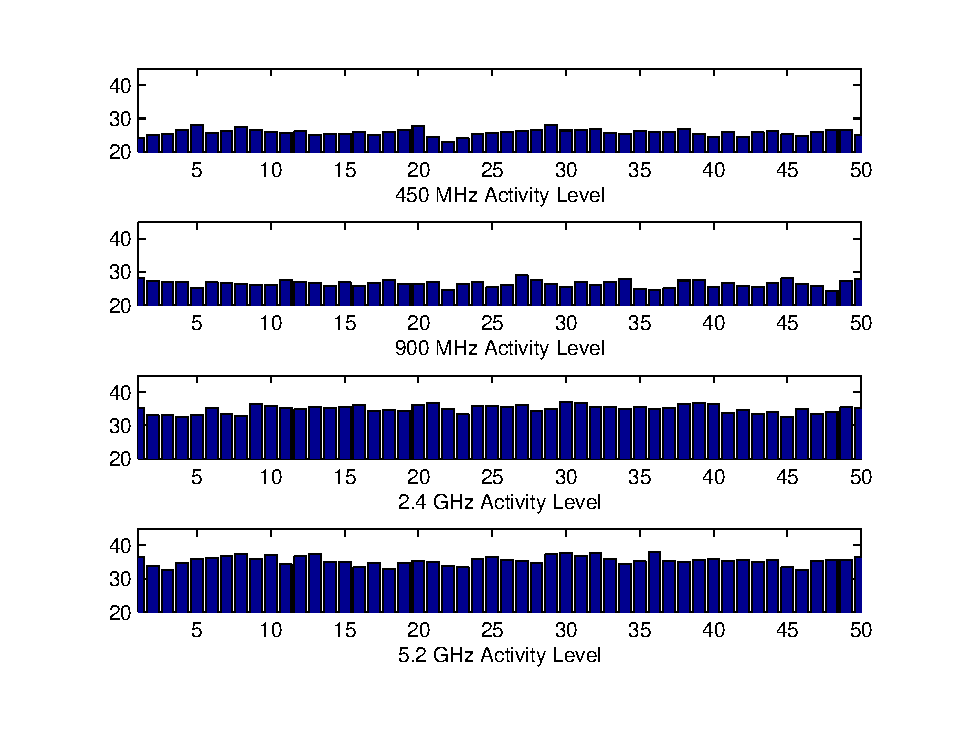
\includegraphics[width=94mm]{figures/labactivity}
%   \vspace{-0.1in}
%   \caption{Wireless Activity in Urban Lab}                                                                 
%   \label{fig:labact}
%   \vspace{-0.1in}
%   \end{figure}
%   
%In the measurements, there is around $10\%$ difference from white space 
%band to WiFi bands in our urban lab. This spectrum utility gap and multiband
%propagation variation in band selection of wireless network 
%deployment is what we have to notice. 
%

\subsection{Model and Problem Formulation}
\label{subsec:problem}

% Assumptions of the network
Oppose to previous works, this paper focuses on bands adaptation of Inter-network 
interference and population density in multiband scenario~\cite{tang2005interference,yuan2006cross
,si2010overview}. We propose a measurement driven framework to get the  
number of access points for serving a certain area with QoS requirement.
We prove that using radios with a greater diversity in propagation could 
achieve overall network performance gains. 
We assume an access point could have limited number of radios, fixed number of 
channels in total, the radios could work in any channel, and the same antenna gain.
Each radio on access point operates with a classic protocol model~\cite{gupta2000capacity}. 
Generally, Internet data request comes with population and Finland government even announce 
broadband is an individual 'legal right'~\cite{bbcfinland,rosston2011household}. 
Providing a community wireless Internet service have to satisfy its traffic demand 
of the people in the area. In populated urban area, more people need more 
network capacity in which case WiFi band spatial reuse is better than white space bands
who limit the capacity in a large area. Moreover, in populated urban area, 
more Inter-network interference comes from TV station and other sources in white space
bands could reduce the capacity of a channel. However, in rural area, too many access points
in WiFi bands for the large area is a waste of funding. Here we are trying to answer the question
 in a certain Inter-network interference, what is the band or bands combination we should 
 use to provide network service for a community with different population density.

Since mathematical formula is difficult to describe the activities of 
signal on the air even in an arbitrary area.
We use long term measurement represent the spectrum utility in each band. 
We define the the percentage of sensing samples $S_\theta$ above a 
interference threshold $\theta$ over the total samples $S$ in a time unit as the 
{\it $Activity Level$} $A$ of Inter-network interference shown in equation~\ref{eq:actdef}
\begin{equation}
\label{eq:actdef}
A=\frac{S_\theta}{S_a}
\end{equation}
The capacity of a clean channel is $C$, with protocol model, the capacity 
of a channel with Inter-network interference $C_r$ could be represented as 
the remaining time multiple the clean channel capacity in equation~\ref{eq:intercap}
\begin{equation}
\label{eq:intercap}
C_r=C*(1-\bar{A})
\end{equation}

A network deployment is suppose to provide network capacity equal to the demand of the service 
area keeping the capacity constraint. The demand of a service area could be calculated as the 
summation of individual demand all over the service area $D_a=\sum_{p\in P}D_p$. Since 
individual or family Internet data demand is marked as government statistics~\cite{rosston2011household}, 
$D_a$ could be remarked with population distribution $f$ and service area $k$ as 
$D_a=\sum_{f \in F,k \in K}\bar{D_p}*f*k$. 
The network deployment capacity constraint could be represented with access points set $M$ 
in equation~\ref{eq:nlbound}

\begin{equation}
\label{eq:nlbound}
\sum_{m \in M}C_r^m \ge \sum_{f \in F,k \in K}\bar{D_p}*f*k
\end{equation}
At the same time, the wireless network has to satisfy the coverage constraint in the service 
area that the access points provide single-hop connectivity for client devices. 
Generally a coverage of $95\%$ is acceptable for outdoor mesh networks~\cite{robinson2010deploying}.

In multiband scenario, the activity level varies with to different interference source 
and the propagation characteristics bring the service area variation due to coverage and 
capacity constraints. A simple method with the least number of access point to cover an area is to use 
multiple orthogonal lower frequency channels. However, FCC limits the white space band utility 
of data communication in most metro area in US~\cite{googledatabase}. Moreover, the number of channels in each 
band is limited. Too many lower frequencies channels will bring huge Intra-network interference for 
the network which is out of our scope. To answer the question given an area for a new network deployment, 
the number of access points which equals to how much funding should be risen, we build the measurement driven
framework {\it Multiband Access Point Estimation} to approach the number of access points for
an arbitrary area.

\begin{algorithm}[t]
\small
\caption{Multiband Access Point Estimation (MAPE)}
\label{algorithm:mape}
\begin{algorithmic}[1]
\REQUIRE  ~~\\
$A$: Measured Activity Level \\
$F$: Population Distribution\\
$C$: Clean Channel Capacity\\
$n$: Path Loss Exponent \\
$B$: Available frequency bands\\
$M$: Area need to be covered
\STATE Chop $M$ in to different type, calculate the traffic demand density $f$
\STATE Calculate in-field channel capacity $C_r$ as $C(1-A)$
\STATE Get the propagation coverage area radius $R_p$ from Frii model based on $n,B,F$
\STATE Calculate the QoS coverage radius $R_{QoS}$ of a Multiband Access Point satisfy the demands of the area
\STATE The coverage radius of a Multiband Access Point is $Min{R_p,R_{QoS}}$
\STATE Apply regular hexagon deployment to get the number of access point for serving given area $M$
\ENSURE ~~\\
The number of Access Points\\
\end{algorithmic}
\end{algorithm}

% Fix the framework , Mark should use them in a single tower with more radios
% Framework
In space domain, the advantage of high frequency channel in network is the spatial reuse, the low
frequency channel is better in large scale coverage. Generally high frequency fit
for populated area and low frequency fit for sparse area.
The time domain variation of spectrum utility across bands could be seen in Figure~\ref{fig:labact}.
For an ISP, the service quality which maps to the capacity constraint has to be satisfied.
Given an area of metropolitan, the population distribution could be found in 
government and academy resources~\cite{uscensus}. Then we have the capacity request
of each part of the area with the assumption everyone has the same Internet demand. 
According to the population distribution, we chop the area into different types.
These are the space domain input. Then we count the measured activity level as 
input in time domain. We have an average channel capacity of each band with the 
activity level. With received signal strength threshold, 
the QoS coverage area of different type per channel and the reuse distance could be computed. 
Then the maximum area an access point could cover can be calculated as the minimize 
area of the QoS coverage area and propagation coverage.
Then the transmitting power is adjusted to fulfill the coverage restriction. 
A classic regular hexagon deployment process is employed to put the access points.

%With this framework, we combine our measurements to evaluate white
%space bands application varying with population density in section~\ref{sec:experimentdesign}.



